% =============================================================================
% CHAPTER 4: Results and Evaluation
% =============================================================================
% SPDX-FileCopyrightText: 2026 Frank Langbein <frank@langbein.org>
% SPDX-License-Identifier: LPPL-1.3c
%
% Suggested sections: Setup (or Evaluation setup / Experimental setup); Results;
% Discussion (or Evaluation and discussion); Limitations. Optional: Ablation
% studies (AI/ML); Comparison with baselines; Threats to validity. Describe how
% you demonstrated the system or hypothesis; include critical tests/experiments;
% critically appraise strengths and weaknesses.
% =============================================================================

\newthought{Tests within a system design project} are inevitable, as they dictate if a project was successful in its aims and has met its requirements. This section will demonstrate what tests were designed for the solution, the results drawn from these tests and will provide an analysis of the project as a whole.

\section{Setup}\label{sec:setup}
% Evaluation setup: data, metrics, baselines, how experiments or tests were run.
% Optional subsections: environment, hyperparameters, evaluation protocol.
Being a combination of a physical device and a software solution, different types of testing had to occur to fully evaluate the performance and accuracy of the solution. The testing conducted was a combination of unit testing and system testing. 

Unit testing was utilised for the modules that can be tested automatically using the \texttt{unit\_test} module in Python. These unit tests can be seen in Algorithms \ref{alg:socketTest} and \ref{alg:playlistTest}. These unit tests also ensured that the shuffle function was called to test if shuffle was passed, the playlist was in fact shuffled.

\begin{algorithm}[!h]
  \caption{socketCommand\_Test - Python}
  \label{alg:socketTest}
  \begin{lstlisting}[language=Python]
    import socket
    import client
    import unittest
    import time
    from unittest.mock import patch

    '''For this unit test, server.py needs to be running'''

    class Test_Socket_Commands(unittest.TestCase):
        def test_play(self):
            response = client.send_command('p')
            self.assertEqual(response, 'Paused/Resumed\n')
        
        def test_skip(self):
            response = client.send_command('s')
            self.assertEqual(response, "Skipped\n")
        
        def test_switch(self):
            response = client.send_command('switch default')
            self.assertEqual(response, "Switching Playlist\n")
            
        def test_invalid_switch(self):
            response = client.send_command('switch akjsdajkhsd')
            self.assertEqual(response, "Playlist not found\n")
            
        def test_help_command(self):
            response = client.send_command('help')
            self.assertTrue(response.startswith("'--------------\nhelp:"))
            
        def test_invalid_command(self):
            response = client.send_command('make sandwich')
            self.assertEqual(response, "Invalid command\n")
            
        def test_null_command(self):
            response = client.send_command('')
            self.assertEqual(response, "Invalid command\n")
            
        # Exit command to be tested manually as order of tests seems to execute exit command first
        # then the rest of the tests (resulting in failure)
  \end{lstlisting}
\end{algorithm}

\begin{algorithm}[!h]
  \caption{loadPlaylist\_Test - Python}
  \label{alg:playlistTest}
  \begin{lstlisting}[language=Python]
    import server
    import random
    import unittest
    from unittest.mock import patch

    class TestLoadPlaylist(unittest.TestCase):
        def test_valid_playlist(self):
            self.assertEqual(server.loadplaylist('default'), True)
            
        def test_invalid_playlist(self):
            self.assertEqual(server.loadplaylist('asjdasdajs'), False)
            
        def test_null_playlist(self):
            self.assertEqual(server.loadplaylist(''), False)
        
        @patch('random.shuffle')
        def test_shuffle_no_args(self, mock_shuffle):
            server.loadplaylist('default')
            self.assertFalse(mock_shuffle.called)
            
        @patch('random.shuffle')
        def test_shuffle_true(self, mock_shuffle):
            server.loadplaylist('default', 'true')
            self.assertTrue(mock_shuffle.called)
            
        @patch('random.shuffle')
        def test_shuffle_false(self, mock_shuffle):
            server.loadplaylist('default', 'false')
            self.assertFalse(mock_shuffle.called)
  \end{lstlisting}
\end{algorithm}
\clearpage

System tests were used for the hardware components of the proposed solution, in this case if the button presses are recognised and audio playing from the correct Bluetooth speaker. The system tests produce results that can be observed but require human interaction, hence why unit tests through Python's \texttt{unittest} module cannot be applied.

The baselines and acceptance criteria for these tests were derived from the functional and non-fuctional requirements, presented in section \ref{sec:spec}.

Testing of the \gls{nfc} module and its reliability was conducted through the use of amending the existing function, documenting:
\begin{itemize}
  \item How many attempts to scan a \gls{nfc} tag have been made.
  \item How many attempts were successful and switched playlists as intended.
\end{itemize}

This was done by creating counters in the form of a list (as they are mutable) that was updated throughout execution. For the function to gain access to these counters, they were passed as arguments and the appropriate \texttt{threading} call was amended to reflect this change. These amendedments can be seen in Algorithms \ref{alg:globalCounters}, \ref{alg:testNFCSwitch} and \ref{alg:NFCReaderCallAmend}.

\begin{algorithm}[!h]
  \caption{Counters for \gls{nfc} Test Snippet - Python}
  \label{alg:globalCounters}
  \begin{lstlisting}[language=Python]
    import time, grovepi, vlc, os, threading, socket, subprocess, serial, re, random

    buttonP_pin = 3 # For some odd reason, the port number + 1 recognises the appropriate button

    buttonS_pin = 8

    grovepi.pinMode(buttonP_pin, "INPUT")
    grovepi.pinMode(buttonS_pin, "INPUT")

    grovepi.digitalWrite(buttonP_pin - 1, 1)

    media_player = vlc.MediaListPlayer() # Intialises Playlist
    instance = vlc.Instance() # Creates VLC instance

    successfulNFCReads = [0] # New Addition
    attemptedNFCReads = [0]
  \end{lstlisting}
\end{algorithm}

\begin{algorithm}[!h]
  \caption{Amended nfc\_reader\_switch() with counter parameters - Python}
  \label{alg:testNFCSwitch}
  \begin{lstlisting}[language=Python]
    def nfc_reader_switch(successfulNFCReads, attemptedNFCReads): # Accetps new arguments
        #Accepting NFC Tags
        serial_port = '/dev/ttyACM0'
        baud_rate = 9600

        ser = serial.Serial(serial_port, baud_rate)

        while True:
            serData = ser.readline().decode('utf-8', errors='ignore')
            if serData.startswith("    Payload"):
                if serData.startswith("    Payload L") == False:
                    print(serData)
                    attemptedNFCReads[0] += 1 # Attempted read occured
                    message = re.findall(r'\.([a-zA-Z]+(?:\s+[a-zA-Z]+)?)', serData)
                    split_msg = message[0].split()
                    media_player.stop()
                    print(attemptedNFCReads)
                    if len(split_msg) == 0:
                        print('Error reading NFC tag, attempt again...')
                    else:
                        if len(split_msg) > 1:
                            loadplaylist(split_msg[0], split_msg[1])
                            successfulNFCReads[0] += 1 # If data extracted successfully, marked as successful
                        else:
                            loadplaylist(message[0])
                            successfulNFCReads[0] += 1
                    media_player.play()
  \end{lstlisting}
\end{algorithm}

\begin{algorithm}[!h]
  \caption{\texttt{threading} call amendment for \gls{nfc} Testing - Python}
  \label{alg:NFCReaderCallAmend}
  \begin{lstlisting}[language=Python]
    if __name__ == '__main__':
        threading2 = threading.Thread(target=nfc_reader_switch, args=(successfulNFCReads, attemptedNFCReads)) # Arguments passed into execution
        threading2.daemon = True
        threading2.start()
  \end{lstlisting}
\end{algorithm}
\newpage
Some preliminary logistical groundwork was also undertaken with the potential of user testing with care home staff with the assistance of ENRICH Cymru. This working relationship was established through visiting a conference with researchers in the field of care home, hosted by Stuart Allen, the project supervisor. Interest was expressed from ENRICH, however complications occurred during application for ethical approval. User testing therefore had to be abandoned for the project to continue ethically, as no response was given in time.
\section{Results}\label{sec:results}
% Main findings: present tables and figures; summarise key outcomes. Optional
% subsections: by research question, by dataset, or by metric.
The results of the test conducted for each component will be split up into corresponding sub-sections with their appropriate figures and test data. In summary, all of the unit tests and system tests passed. This was largely due to the testing spearheading development, encouraging error checking throughout to keep the system as reliable as possible.

\subsection{Terminal Command Testing Results}\label{subsec:terminalResults}
This module was evaluated using unit tests to see if the appropriate output was returned through the terminal. As seen in algorithm \ref{alg:socketTest}, each possible command bar the \texttt{exit} command has been set up as an automatic test, as the \texttt{exit} command was tested in isolation. Results of the tests are seen in Table \ref{tab:terminalResults}

\begin{table}[!h]
  \centering
  \caption{Terminal Commands Testing Table}
  \label{tab:terminalResults}
  \begin{tabularx}{\linewidth}{llXXl}
    \toprule
    Type of Testing Data & Input & Expected Output & Actual Output & Pass/Fail \\ \hline
    \midrule
    Normal & p & Song Paused & Song Paused & Pass \\ \hline
    Normal & s & Song Skipped & Song Skipped & Pass \\ \hline
    Normal & switch default & Switching Playlist & Switching Playlist & Pass \\ \hline
    Normal & switch default true & Switching Playlist & Switching Playlist & Pass \\ \hline
    Normal & exit & Exiting & Exiting & Pass \\ \hline
    Erroneous & x & Throws Error and prompts reinput & Throws Error and prompts reinput & Pass \\ \hline
    Erroneous & f & Throws Error and prompts reinput & Throws Error and prompts reinput & Pass \\ \hline
    Erroneous & switch asjdashd & Playlist not found & Playlist not found & Pass \\ \hline
    Null & N/A & Throws Error and prompts reinput & Throws Error and prompts reinput & Pass \\ \hline
    \bottomrule
  \end{tabularx}
\end{table}

All of the results returned a pass with handling all the types of data that could be passed into the terminal.
\clearpage
\subsection{Button Interaction Testing Results}\label{subsec:btnResults}
This module was evaluated using system tests as human input was necessary so automated unit tests were impractical to enact. The results for these tests can be seen in Table \ref{tab:buttonResults}.

\begin{table}[!h]
  \centering
  \caption{Button Interaction Testing Table}
  \label{tab:buttonResults}
  \begin{tabular}{lllll}
    \toprule
    Type of Testing Data & Input & Expected Output & Actual Output & Pass/Fail \\
    \midrule
    Normal & D2 button press & Song Paused & Song Paused & Pass \\
    Normal & D7 button press & Song Skipped & Song Skipped & Pass \\
    Erroneous & D3 button press & Nothing happens & Nothing happens & Pass \\
    Erroneous & D5 button press & Nothing happens & Nothing happens & Pass \\
    Null & N/A & Nothing happens & Nothing happens & Pass \\
    \bottomrule
  \end{tabular}
\end{table}
All of these system tests returned a pass with all of the documented button interactions, including inputs from mismatched port numbers. 

\subsection{Loading Playlist Testing Results}\label{subsec:playlistResults}
Being a self-contained function that did not require human interaction during its testing process, \texttt{load\_playist()} was a perfect candidate for the Python \texttt{unittest} module. The preconstructed unit tests attempts to load the \texttt{default} playlist with and without the \texttt{shuffle} parameter present. The results can be seen in Table \ref{tab:loadPlaylistTest}.
\begin{table}[!h]
  \centering
  \caption{load\_playlist() Testing Table}
  \label{tab:loadPlaylistTest}
  \begin{tabular}{lllll}
    \toprule
    Type of Testing Data & Input & Expected Output & Actual Output & Pass/Fail \\
    \midrule
    Normal & \texttt{default} & True & True & Pass \\
    Normal & \texttt{default} & Shuffle Not Called & Shuffle Not Called & Pass \\
    Normal & \texttt{default false} & Shuffle Not Called & Shuffle Not Called & Pass \\
    Normal & \texttt{default true} & Shuffle Called & Shuffle Called & Pass \\
    Erroneous & \texttt{asjdasdajs} & False & False & Pass \\
    Null & N/A & False & False & Pass \\
    \bottomrule
  \end{tabular}
\end{table}
All of the unit tests for this function were able to pass, demonstrating how the function is to behave. 
\subsection{NFC System Testing Results}\label{subsec:NFCResults}
The \gls{nfc} module also required human interaction during the testing process so was subject to system tests, instead of unit tests. The process of the test was to leave a \gls{nfc} tag onto the antenna for 100 cycles of scanning the tag and see what percentage scans were successful. The results of this test are visible in Table \ref{tab:NFCScanResults}
\clearpage
\begin{table}[!h]
  \centering
  \caption{\gls{nfc} Scan Robustness Testing Data}
  \label{tab:NFCScanResults}
  \begin{tabular}{llll}
    \toprule
    \gls{nfc} Tag Content & Attempted \gls{nfc} Scans & Successful \gls{nfc} Scans & Success Rate (\%)  \\
    \midrule
    \texttt{default} & 100 & 100 & 100\% \\
    \texttt{backrooms} & 100 & 100 & 100\% \\
    \texttt{jazz} & 100 & 100 & 100\% \\
    \bottomrule
  \end{tabular}
\end{table}

All of these preregistered \gls{nfc} tags were read at a 100\% success rate and enacted their appropriate playlist switch each time they were scanned.

\subsection{Response Time Testing Results}\label{subsec:execTimeResults}
Response Times for various components (including scalability of the playlists sizes) of the proposed solution were tested using either a stopwatch as execution occurred (in the case of time taken for the main script to be ran at boot, denoted by the predefined speaker playing the first song) or utilising the \texttt{time} command on Linux and taking the \texttt{real} value, as it represents the real time between invocation and execution. 

Scalability was tested through a larger playlist named \texttt{bigplaylist} that contained three times the amount of songs in comparison to the three playlists created through development. The detailed timings for each of these can be seen in the appendix \ref{app:results} but an abridged version containing the averages can be seen in Table \ref{tab:avgResTime}.
\begin{table}[!h]
  \centering
  \caption{Average Response Time for Components}
  \label{tab:avgResTime}
  \begin{tabularx}{\linewidth}{XlXl}
    \toprule
    Component Tested & Average Time Taken (s) & Associated Requirement & Pass/Fail \\
    \midrule
    Load Script on Boot & 34.9s & Non-functional Requirement \ref{req:startupTime} & Pass \\ \hline
    Skip Song Execute & 0.1454s & Non-functional Requirement \ref{req:remoteTime} & Pass \\ \hline
    Pause/Play Song Execute & 0.1434s & Non-functional Requirement \ref{req:remoteTime} & Pass \\ \hline
    Switch Playlist Execute & 0.1437s & Non-functional Requirement \ref{req:remoteTime} & Pass \\ \hline
    Switch with Shuffle Execute & 0.1472s & Non-functional Requirement \ref{req:remoteTime} & Pass \\ \hline
    Switch Large Playlist Execute & 0.1416s & Non-functional Requirement \ref{req:scalability} & Pass \\ \hline
    Switch Large Playlist with Shuffle Execute & 0.141s & Non-functional Requirement \ref{req:scalability} & Pass \\ \hline
    \bottomrule
  \end{tabularx}
\end{table}

On average, terminal code execution took approximately 0.144s to execute. Including boot behaviour, average code execution is estimated to be 5.109s.

\subsection{Security Testing Results}\label{subsec:secureResults}
Lastly, the final component to be tested through system testing was the remote solutions authentication methods. Here, two users attempt to connect to the proposed solution using made-up credentials and are not allowed access to the \gls{ssh} terminal, pictured in Figures \ref{fig:noUser1} and \ref{fig:noUser2}.

\begin{figure}[!h]
  \centering
  \fbox{\rule{0pt}{3.7cm}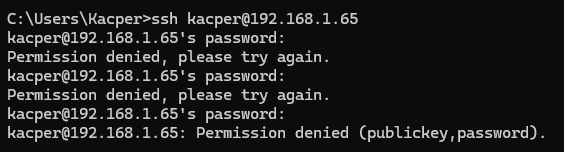
\includegraphics[width=0.97\textwidth]{images/nouser1}}
  \caption[Incorrect Credentials]{Incorrect Credentials - user 'kacper'}\label{fig:noUser1}
\end{figure}

\begin{figure}[!h]
  \centering
  \fbox{\rule{0pt}{3.5cm}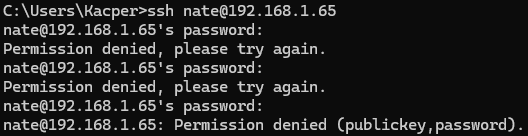
\includegraphics[width=0.97\textwidth]{images/nouser2}}
  \caption[Incorrect Credentials]{Incorrect Credentials - user 'nate'}\label{fig:noUser2}
\end{figure}

As the users are not able to access the \gls{ssh} terminal with incorrect credentials, the test is given a pass.

\section{Discussion}\label{sec:discussion}
% Critical appraisal: strengths, weaknesses, methodology choices; comparison
% with prior work. Optional: ablation analysis, sensitivity analysis.
This section will address the strengths and weaknesses of the proposed solution, highlighting methodological choices and why they were chosen along the way.

\subsection{Strengths}\label{subsec:strengths}
The proposed solution throughout was testing was largely successful. One of the key strengths that helped contribute to the systems success was reliably being able to connect to the system remotely. As demonstrated through testing, the system is able to be interfaced with and managed entirely remotely, with no necessary physical interaction. The commands sent through the remote interface are fast and execute all the necessary actions a media player requires. The remote solution is also not limited to just a Command Line Interface, as users are able to connect using \gls{vnc} if they prefer a graphical interface. This directly addresses the main objective of the remote management for the system and through testing, it is strongly suggested that the system is efficient with its remote communication.

Simplicity in its physical implementation strengths the belief the system is successful. As backed by research conducted in section \ref{subsec:medContext} and the informal chat with ENRICH Cymru, this was the most important aspect of the implementation. The system provides a simple \gls{ui} through its remote solution, but omits one through its hardware, presenting only two simple buttons to perform two simple actions. Avoiding over-complicating the device ensured that the main stakeholders were still the focus throughout development, creating a truly tailored solution for the cognitively impaired.

Finally, the system addresses an important aspect of life that may be missed in assistive technologies for the cognitively impaired, especially patients with dementia. The neglect of making leisure accessible is apparent, considering the positive impact that it has on the mental wellbeing of dementia patients. The focus on delivering music in an accessible manner tackles this unexplored market of accessible technologies and provides a proof of concept that technology can be designed with accessibility embedded in its development. This is a strength as it highlights a disparity within the field of assistive technologies focusing mostly on care and extending 'quantity of life', rather than 'quality of life'.  

\subsection{Weaknesses}\label{subsec:weaknesses}
The proposed solution is not without its flaws. For instance, although the system is intended to run completely offline, it does require a constant internet connection to be able to interface with it remotely, either through \gls{ssh} or \gls{vnc}. The alternative would be to manage the system offline but this would require a constant keyboard, mouse and monitor to be connected to the device. This could be mitigated if given more time and resources but the current state of the proposed solution requires a constant internet connection.

Being a device tailored towards simplicty, the inital setup of the device is complex and does require a level of technical knowledge to enact. Should the proposed solution come packaged with the correct prerequisites, a mouse, keyboard and monitor are still required to ensure that the device can be connected to a new network to enable remote management. Connection to this new network then imposes its own \gls{dhcp} protocol onto the proposed solution and assigns it a new IP address. Even if a static IP address was assigned beforehand, there is no guarantee that the IP address hasn't already been taken by another device or if the device used to \gls{ssh} onto the proposed solution is in the same subnet and can contact the proposed solution. This could as well be mitigated if given more time and resources.

Finally, \gls{nfc}, one of the main features and methods of interaction, requires a level of setup that isn't intuitive. This is primarily due to a lack of testing on alternatives, however, there only exists one supported way of writing to the \gls{nfc} tags. The script on the Arduino must be switched to an alternative writing script and then switched back to the reading script before the \gls{nfc} functionality is restored to the proposed solution. The switching of the scripts requires a separate device that has access to the Arduino IDE and the accompanying Arduino library that contains the functionality to interface with PN532 devices, that being the \gls{nfc} module. This would have to occur each time a new playlist (or if the playlist is to be shuffled or not) has been added to the proposed solution if the user wishes for all the playlists to be available using \gls{nfc}. This undermines the simplicity of the device if such intricate setup processes are necessary beforehand. 

\subsection{Methodology Choices}\label{subsec:methodology}
The project was completed utilising a Waterfall Methodology throughout its development. This was set out by the inital plan that was completed prior to the start of this project, where clear deliverables were identified and milestones generated. Each feature was developed in a vacuum week by week in its entirety until it was integrated into the system at large. This methodology did remain flexible to allow for buffers between features if development took longer than expected or bugs were identified within the modules.

The predictability within the Waterfall Model was beneficial as it helped keep discussions with the project supervisor directed, it ensured that each week quantifiable progress can be observed and time could be effectively managed based on progress as each feature was given a predetermined time slot that was open for alteration.